\section{Summary}
\subsection{Discussion}
\begin{frame}
    \frametitle{Discussion}
\begin{itemize}
 \item MD simulations is a powerful method buth with limitations due to force field accuracy and computational demands. Integrative modeling approaches may be used to tackle the limitations.

\item Logic is following: while modeling structural elements and parameters that are sensitive to force field accurace additional experimental restraints should be used. Conformationally robust elements may be modeled using conventional approaches.

\item Symmetry considerations and multi-scale modeling approaches can be used to further extend the limits.
\end{itemize}


\end{frame}

\subsection{Conclusions}
\begin{frame}%[allowframebreaks]
    \frametitle{Conclusions}

\begin{enumerate}
\justifying
\scriptsize
%\tiny
% \fontsize{5}{6}
\item An integrative approach and software solutions for multiscale modeling of DNA and protein complexes have been developed, which uses various experimental data on DNA footprinting, electron microscopy, FRET microscopy and a combined representation of DNA in the atomistic and dinucleotide approximations.


  \item In the microsecond time range, the parameters of large-scale functional conformational changes in the structure of nucleosomes were determined: the ensemble of conformations of the linker DNA was calculated, the effect of electrostatic repulsion on the geometry of the linker DNA segments was determined, the characteristic time of dissociation of the ends of the nucleosomal DNA from the histone octamer (10 $\mu$s) was determined, and fluctuation structural mechanisms of the formation of defect formation were determined. twisting DNA, switching the conformations of histone tails.



  \item The processing of experimental data on DNA cleavage by hydroxyl radicals (DNA footprinting) made it possible to calculate the probability of DNA cleavage for each nucleotide. It was shown that the profiles of DNA cleavage by hydroxyl radicals in the nucleosome depend little on the DNA sequence and are mainly determined by the positioning of DNA on the nucleosome. An algorithm is proposed for the precise determination of the position of DNA in the nucleosome from footprinting data for two DNA strands based on the position of the pseudosymmetry axis.

\end{enumerate}
\end{frame}

\begin{frame}%[allowframebreaks]
    \frametitle{Conclusions (continued)}

\begin{enumerate}
\justifying
\scriptsize
%\tiny
% \fontsize{5}{6}

  \item Using integrative modeling methods, the structures and parameters of interactions of nucleosome complexes with RNA polymerases, CENP-C protein, histone H1, and proteins of the FACT complex were established. It was found that at position +49, after entering the nucleosome, RNA polymerase II can form a compact complex with the nucleosome, in which contacts of histones with DNA are retained on both sides of the active site. In the model of the centromeric nucleosome of yeast, the position of DNA was determined and it was found that the CENP-C protein interacts with the nucleosome in the region of 20 nucleotides from the center of symmetry of the nucleosome. Models of the conformation of linker DNA segments during histone H1 binding are proposed. The amplitudes of the conformational mobility of DNA in nucleosomes upon binding to the FACT complex were determined.
  

 \item The developed approaches to constructing models of amyloid-like fibrils made it possible to study the relationship of the mutual arrangement of peptides in fibrillar structures with the large-scale morphology of amyloid-like fibrils and thus to establish the structural organization of filaments based on diblock oligomers of quaterthiophene and peptide $(Thr-Val)_3$ protein, as well as on the basis of the gp120 protein. It was found that the considered amyloid-like fibrils can be formed on the basis of two interacting beta sheets, which form either a flat ribbon or a left-handed ribbon with a period of 24-30 nm.

\end{enumerate}
\end{frame}

% \begin{frame}
%     \frametitle{Научная новизна}
%     \begin{itemize}
%         \item Впервые реализован \dots
%         \item Разработана программа \dots
%         \item Впервые проведён анализ \dots
%         \item Предложена схема \dots
%     \end{itemize}
% \end{frame}
% \note{
%     Проговаривается вслух научная новизна
% }

% \begin{frame}
%     \frametitle{Научная и практическая значимость}
%     \begin{itemize}
%         \item Получены выражения для \dots.
%         \item Определены условия \dots.
%         \item Разработаны устройства \dots.
%     \end{itemize}
% \end{frame}
% \note{
%     Проговариваются вслух научная и практическая значимость
% }

% \begin{frame}
%     \frametitle{Свидетельство о регистрации программы}
%     \begin{figure}[h]
%         \centering
%         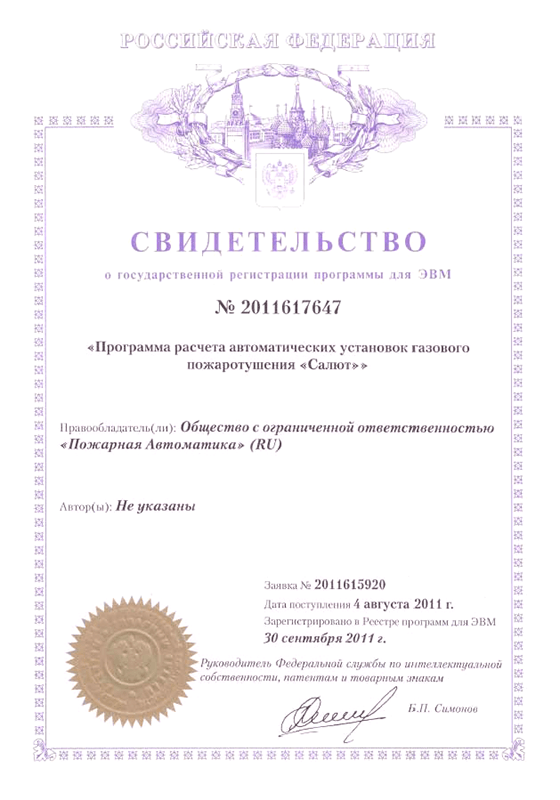
\includegraphics[height=0.7\textheight]{registration}
%     \end{figure}
% \end{frame}
% \note{
%     Получено свидетельство о регистрации разработанной программы \textsc{Hello~world™}.
% }

% \begin{frame}
%     \frametitle{Акт о внедрении}
%     \begin{figure}[h]
%         \centering
%         \fbox{
%             \begin{minipage}[t]{0.4\linewidth}
%                 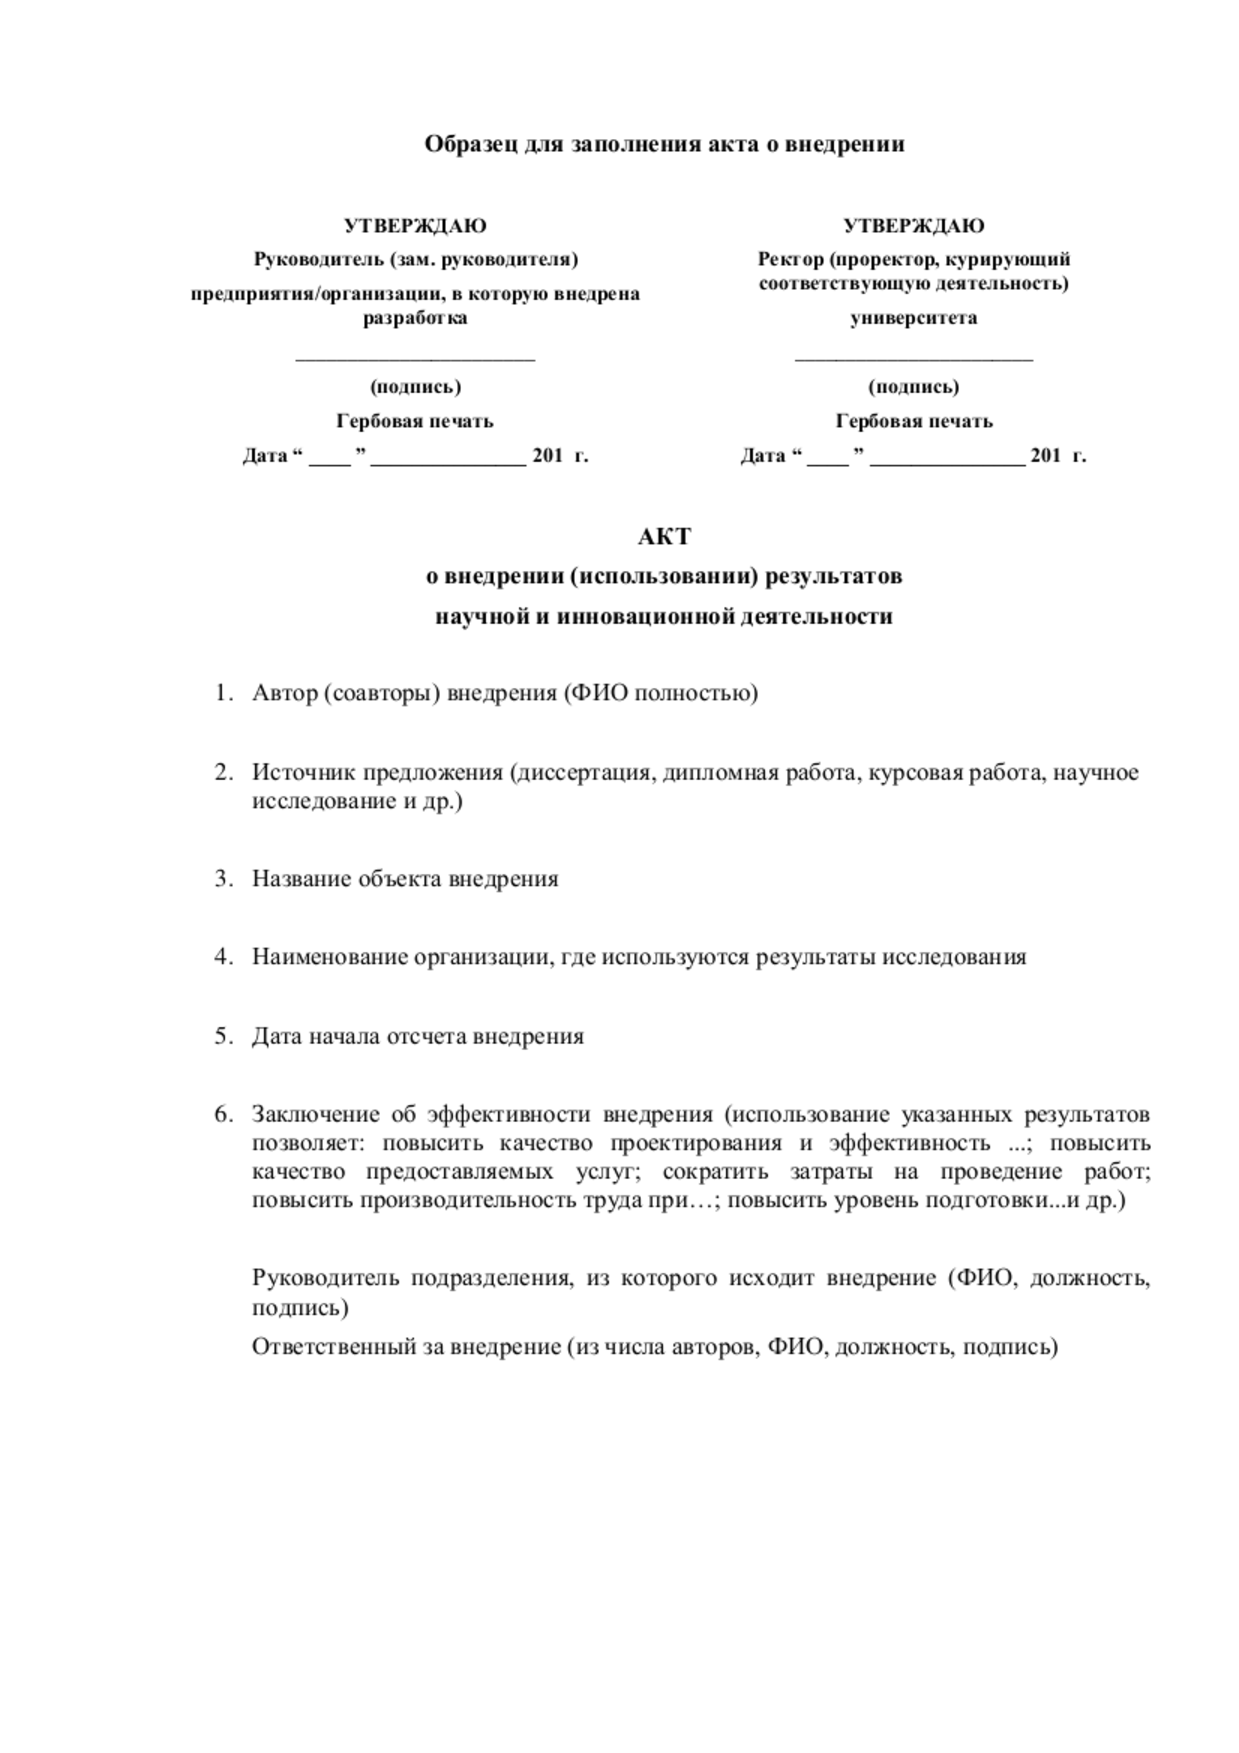
\includegraphics[width=\linewidth]{implementation}
%             \end{minipage}
%         }
%     \end{figure}
% \end{frame}
% \note{
%     Получен акт о внедрении.
% }
\subsection{Key publications}
\begin{frame}[allowframebreaks] % публикации на одной странице
% \begin{frame}[t,allowframebreaks] % публикации на нескольких страницах
    \frametitle{Key publications}
% \nocite{hada_histone_2019,bass_effect_2019,armeev_linking_2019,shaytan_structural_2018,gorkovets_joint_2018,xiao_molecular_2017,shaytan_hydroxyl-radical_2017,gribkova_investigation_2017,el_kennani_ms_histonedb_2017,chertkov_dual_2017,armeev_modeling_2016,armeev_nucleosome_2016,biswas_genomic_2016,draizen_histonedb_2016,lyubitelev_structure_2016,shaitan_dynamics_2016,shaytan_coupling_2016,shaytan_trajectories_2016,valieva_large-scale_2016,armeev_conformational_2015,armeev_molecular_2015,frank_direct_2015,gaykalova_structural_2015,goncearenco_structural_2015,shaytan_nucleosome_2015,bozdaganyan_comparative_2014,chang_analysis_2014,kasimova_voltage-gated_2014,nishi_physicochemical_2014,sokolova_genome_2014,yolamanova_peptide_2013,shaitan_influence_2013,orekhov_calculation_2012,shaytan_self-assembling_2011,shaytan_self-organizing_2011}
% \renewcommand*{\bibfont}{\normalfont\scriptsize}
% %\renewcommand\bibliographytypesize{\small}
%     \ifnumequal{\value{bibliosel}}{0}{
%         \insertbiblioauthor
%     }{
%         \printbibliography%
%     }

\setbeamertemplate{enumerate items}[default]
\setbeamercolor*{enumerate item}{fg=black}
\scriptsize
\begin{enumerate}
 \justifying

 \item Histone Octamer Structure Is Altered Early in ISW2 ATP-Dependent Nucleosome Remode-ling / A. Hada, S. K. Hota, J. Luo, Y.-c. Lin, S. Kale, A. K. Shaytan, S. K. Bhardwaj, [et al.] // Cell Reports. –– 2019. –– July 2. –– Vol. 28, no. 1. –– 282––294.e6. –– DOI: 10.1016/j.celrep.2019. 05.106. –– \textbf{IF WoS 7.7} - (2,3/0,3).
\item The Effect of Oncomutations and Posttranslational Modifications of Histone H1 on Chroma-tosome Structure and Stability / M. V. Bass, G. A. Armeev, K. V. Shaitan, A. K. Shaytan // Moscow University Biological Sciences Bulletin. –– 2019. –– July. –– Vol. 74, no. 3. –– P. 121––126. –– DOI: 10.3103/S0096392519030015. –– \textbf{IF RINC 0.76} - (0,7/0,3).
\item  Linking Chromatin Composition and Structural Dynamics at the Nucleosome Level / G. A. Armeev, A. K. Gribkova, I. Pospelova, G. A. Komarova, A. K. Shaytan // Current Opinion in Structural Biology. –– 2019. –– June. –– Vol. 56. –– P. 46––55. –– DOI: 10.1016/j.sbi. 2018.11.006. –– \textbf{IF WoS 6.908} - (1,2/0,6).
\item  Structural Interpretation of DNA–Protein Hydroxyl-Radical Footprinting Experiments with High Resolution Using HYDROID / A. K. Shaytan, H. Xiao, G. A. Armeev, D. A. Gaykalova, G. A. Komarova, C. Wu, V. M. Studitsky, D. Landsman, A. R. Panchenko // Nature Protocols. –– 2018. –– Nov. –– Vol. 13, no. 11. –– P. 2535––2556. –– DOI: 10.1038/s41596-018-0048-z. –– \textbf{IF WoS 11.334} - (2,5/2,2).
\item  Joint Effect of Histone H1 Amino Acid Sequence and DNA Nucleotide Sequence on the Structure of Chromatosomes: Analysis by Molecular Modeling Methods / T. K. Gorkovets, G. A. Armeev, K. V. Shaitan, A. K. Shaytan // Moscow University Biological Sciences Bulletin. –– 2018. –– Apr. –– Vol. 73, no. 2. –– P. 82––87. –– DOI: 10 . 3103 / S0096392518020025. –– \textbf{IF RINC 0.76} - (0,7/0,3).
\item  Molecular Basis of CENP-C Association with the CENP-A Nucleosome at Yeast Centromeres / H. Xiao, F. Wang, J. Wisniewski, A. K. Shaytan, R. Ghirlando, P. C. FitzGerald, Y. Huang, [et al.] // Genes \& Development. –– 2017. –– Oct. 1. –– Vol. 31, no. 19. –– P. 1958––1972. –– DOI: 10.1101/gad.304782.117. –– \textbf{IF WoS 9.527} - (1,7/0,3).
\item  Hydroxyl-Radical Footprinting Combined with Molecular Modeling Identifies Unique Features of DNA Conformation and Nucleosome Positioning / A. K. Shaytan, H. Xiao, G. A. Armeev, C. Wu, D. Landsman, A. R. Panchenko // Nucleic Acids Research. –– 2017. –– Sept. 19. –– Vol. 45, no. 16. –– P. 9229––9243. –– DOI: 10.1093/nar/gkx616. –– \textbf{IF WoS 11.501} - (1,7/1,5).
\item  Gribkova, A. K. Investigation of Histone-DNA Binding Energy as a Function of DNA Unwrapping from Nucleosome Using Molecular Modeling / A. K. Gribkova, G. A. Armeev, A. K. Shaytan // Moscow University Biological Sciences Bulletin. –– 2017. –– July. –– Vol. 72, no. 3. –– P. 142––145. –– DOI: 10.3103/S009639251703004X. –– \textbf{IF RINC 0.76} - (0,5/0,2).
\item  MS\_HistoneDB, a Manually Curated Resource for Proteomic Analysis of Human and Mouse Histones / S. El Kennani, A. Adrait, A. K. Shaytan, S. Khochbin, C. Bruley, A. R. Panchenko, D. Landsman, D. Pflieger, J. Govin // Epigenetics \& Chromatin. –– 2017. –– Dec. –– Vol. 10, no. 1. –– DOI: 10.1186/s13072-016-0109-x. –– \textbf{IF WoS 5.333} - (2,1/0,5).
\item  Dual Active Site in the Endolytic Transglycosylase Gp144 of Bacteriophage phiKZ / O. V. Chertkov, G. A. Armeev, I. V. Uporov, S. A. Legotsky, N. N. Sykilinda, A. K. Shaytan, N. L. Klyachko, K. A. Miroshnikov // Acta Naturae. –– 2017. –– Vol. 9, no. 1. –– P. 7. –– DOI: 10.32607/20758251-2017-9-1-81-87. –– \textbf{IF WoS 1.62} - (0,8/0,1).
\item  Modeling of the Structure of Protein–DNA Complexes Using the Data from FRET and Footprinting Experiments / G. A. Armeev, T. K. Gorkovets, D. A. Efimova, K. V. Shaitan, A. K. Shaytan // Moscow University Biological Sciences Bulletin. –– 2016. –– Jan. –– Vol. 71, no. 1. –– P. 29––33. –– DOI: 10.3103/S0096392516010016. –– \textbf{IF RINC 0.76} - (0,6/0,2).
\item  Armeev, G. A. Nucleosome Structure Relaxation during DNA Unwrapping: Molecular Dynamics Simulation Study / G. A. Armeev, K. V. Shaitan, A. K. Shaytan // Moscow University Biological Sciences Bulletin. –– 2016. –– July. –– Vol. 71, no. 3. –– P. 141––144. –– DOI: 10.3103/S0096392516030020. –– \textbf{IF RINC 0.76} - (0,5/0,2).
 \item  Genomic Profiling of Multiple Sequentially Acquired Tumor Metastatic Sites from an “Exceptional Responder” Lung Adenocarcinoma Patient Reveals Extensive Genomic Hetero-geneity and Novel Somatic Variants Driving Treatment Response / R. Biswas, S. Gao, C. M. Cultraro, T. K. Maity, A. Venugopalan, Z. Abdullaev, A. K. Shaytan, [et al.] // Molecular Case Studies. –– 2016. –– Nov. –– Vol. 2, no. 6. –– a001263. –– DOI: 10.1101/mcs.a001263. –– \textbf{IF WoS 1.750} - (3,1/0,5).
 \item  HistoneDB 2.0: A Histone Database with Variants—an Integrated Resource to Explore Histones and Their Variants / E. J. Draizen, A. K. Shaytan, L. Marino-Ramirez, P. B. Talbert, D. Landsman, A. R. Panchenko // Database. –– 2016. –– Vol. 2016. –– baw014. –– DOI: 10.1093/database/baw014. –– \textbf{IF WoS 2.593} - (1,2/0,6).
 \item  Structure and Functions of Linker Histones / A. V. Lyubitelev, D. V. Nikitin, A. K. Shaytan, V. M. Studitsky, M. P. Kirpichnikov // Biochemistry (Moscow). –– 2016. –– Mar. –– Vol. 81, no. 3. –– P. 213––223. –– DOI: 10.1134/S0006297916030032. –– \textbf{IF WoS 1.978} - (1,3/0,1).
 \item  Shaitan, K. V. The Dynamics of Irreversible Evaporation of a Water–Protein Droplet and the Problem of Structural and Dynamic Experiments with Single Molecules / K. V. Shaitan, G. A. Armeev, A. K. Shaytan // Biophysics. –– 2016. –– Mar. –– Vol. 61, no. 2. –– P. 177––184. –– DOI: 10.1134/S0006350916020172. –– \textbf{IF SJR 0.226} - (0,9/0,1).
 \item  Coupling between Histone Conformations and DNA Geometry in Nucleosomes on a Micro-second Timescale: Atomistic Insights into Nucleosome Functions / A. K. Shaytan, G. A. Armeev, A. Goncearenco, V. B. Zhurkin, D. Landsman, A. R. Panchenko // Journal of Molecular Biology. –– 2016. –– Jan. –– Vol. 428, no. 1. –– P. 221––237. –– DOI: 10.1016/j.jmb.2015.12.004. –– \textbf{IF WoS 5.04} - (2,0/1,8).
 \item  Trajectories of Microsecond Molecular Dynamics Simulations of Nucleosomes and Nucleo-some Core Particles / A. K. Shaytan, G. A. Armeev, A. Goncearenco, V. B. Zhurkin, D. Landsman, A. R. Panchenko // Data in Brief. –– 2016. –– June. –– Vol. 7. –– P. 1678––1681. –– DOI: 10.1016/j.dib.2016.04.073. –– \textbf{IF WoS 0.97} - (0,5/0,5).
 \item  Large-Scale ATP-Independent Nucleosome Unfolding by a Histone Chaperone / M. E. Valieva, G. A. Armeev, K. S. Kudryashova, N. S. Gerasimova, A. K. Shaytan, O. I. Kulaeva, L. L. McCullough, [et al.] // Nature Structural \& Molecular Biology. –– 2016. –– Dec. –– Vol. 23, no. 12. –– P. 1111––1116. –– DOI: 10.1038/nsmb.3321. –– \textbf{IF WoS 11.98} - (0,9/0,1).
 \item  Armeev, G. A. Conformational Flexibility of Nucleosomes: A Molecular Dynamics Study / G. A. Armeev, K. V. Shaitan, A. K. Shaytan // Moscow University Biological Sciences Bulletin. –– 2015. –– July. –– Vol. 70, no. 3. –– P. 147––151. –– DOI: 10.3103/S009639251- 5030025. –– \textbf{IF RINC 0.76} - (0,6/0,3).
 \item  Armeev, G. A. Molecular Dynamics Study of the Ionic Environment and Electrical Character-istics of Nucleosomes / G. A. Armeev, K. V. Shaitan, A. K. Shaitan // Moscow University Biological Sciences Bulletin. –– 2015. –– Oct. –– Vol. 70, no. 4. –– P. 173––176. –– DOI: 10.3103/ S0096392515040033. –– \textbf{IF RINC 0.76} - (0,5/0,2).
 \item  Direct Prediction of Residual Dipolar Couplings of Small Molecules in a Stretched Gel by Stochastic Molecular Dynamics Simulations: Direct Prediction of Residual Dipolar Couplings by Stochastic MD Simulations / A. O. Frank, J. C. Freudenberger, A. K. Shaytan, H. Kessler, B. Luy // Magnetic Resonance in Chemistry. –– 2015. –– Mar. –– Vol. 53, no. 3. –– P. 213––217. –– DOI: 10.1002/mrc.4181. –– \textbf{IF WoS 1.731} - (0,6/0,1).
 \item  Structural Analysis of Nucleosomal Barrier to Transcription / D. A. Gaykalova, O. I. Kulaeva, O. Volokh, A. K. Shaytan, F.-K. Hsieh, M. P. Kirpichnikov, O. S. Sokolova, V. M. Studitsky // Proceedings of the National Academy of Sciences. –– 2015. –– Oct. 27. –– Vol. 112,
no. 43. –– E5787––E5795. –– DOI: 10.1073/pnas.1508371112. –– \textbf{IF WoS 9.412} - (1,0/0,3).
 \item  Structural Perspectives on the Evolutionary Expansion of Unique Protein-Protein Binding Sites / A. Goncearenco, A. K. Shaytan, B. A. Shoemaker, A. R. Panchenko // Biophysical Journal. –– 2015. –– Sept. –– Vol. 109, no. 6. –– P. 1295––1306. –– DOI: 10.1016/j.bpj.2015. 06.056. –– \textbf{IF WoS 3.665} - (1,4/0,4).
 \item  Shaytan, A. K. Nucleosome Adaptability Conferred by Sequence and Structural Variations in Histone H2A-H2B Dimers / A. K. Shaytan, D. Landsman, A. R. Panchenko // Current Opinion in Structural Biology. –– 2015. –– June. –– Vol. 32. –– P. 48––57. –– DOI: 10.1016/j.sbi. 2015.02.004. –– \textbf{IF WoS 6.908} - (1,2/1,0).
 \item  Comparative Computational Study of Interaction of C60-Fullerene and Tris-Malonyl-C60- Fullerene Isomers with Lipid Bilayer: Relation to Their Antioxidant Effect / M. E. Bozdaga-nyan, P. S. Orekhov, A. K. Shaytan, K. V. Shaitan // PLoS ONE / ed. by C. M. Soares. –– 2014. –– July 14. –– Vol. 9, no. 7. –– e102487. –– DOI: 10.1371/journal. pone.0102487. –– \textbf{IF WoS 2.740} - (0,9/0,1).
 \item  Analysis of the Mechanism of Nucleosome Survival during Transcription / H.-W. Chang, O. I. Kulaeva, A. K. Shaytan, M. Kibanov, K. Kuznedelov, K. V. Severinov, M. P. Kirpichnikov, D. J. Clark, V. M. Studitsky // Nucleic Acids Research. –– 2014. –– Feb. –– Vol. 42,
no. 3. –– P. 1619––1627. –– DOI: 10 . 1093 / nar / gkt1120. –– \textbf{IF WoS 11.501} - (1,0/0,2).
 \item  Voltage-Gated Ion Channel Modulation by Lipids: Insights from Molecular Dynamics Simulations / M. A. Kasimova, M. Tarek, A. K. Shaytan, K. V. Shaitan, L. Delemotte // Biochimica et Biophysica Acta (BBA) - Biomembranes. –– 2014. –– May. –– Vol. 1838, no. 5. –– P. 1322––1331. –– DOI: 10.1016/j.bbamem.2014.01.024. –– \textbf{IF WoS 3.4} - (1,2/0,1).
 \item  Nishi, H. Physicochemical Mechanisms of Protein Regulation by Phosphorylation / H. Nishi, A. Shaytan, A. R. Panchenko // Frontiers in Genetics. –– 2014. –– Aug. 7. –– Vol. 5. –– DOI: 10.3389/fgene.2014. 00270. –– \textbf{IF WoS 3.789} - (1,2/0,4).
 \item  Genome Packaging in EL and Lin68, Two Giant phiKZ-like Bacteriophages of P. Aeruginosa / O. Sokolova, O. Shaburova, E. Pechnikova, A. Shaytan, S. Krylov, N. Kiselev, V. Krylov // Virology. –– 2014. –– Nov. –– Vol. 468––470. –– P. 472––478. –– DOI: 10.1016/j.virol.2014.09. 002. –– \textbf{IF WoS 2.464} - (0,8/0,1).
 \item  Peptide Nanofibrils Boost Retroviral Gene Transfer and Provide a Rapid Means for Concent-rating Viruses / M. Yolamanova, C. Meier, A. K. Shaytan, V. Vas, C. W. Bertoncini, F. Arnold, O. Zirafi, [et al.] // Nature Nanotechnology. –– 2013. –– Feb. –– Vol. 8, no. 2. –– P. 130––136. –– DOI: 10.1038/nnano.2012.248. –– \textbf{IF WoS 31.538} - (0,8/0,2).
 \item  Influence of Interionic Interactions on Functional State and Blocker Binding of Voltage-Gated Potassium Channels / K. V. Shaitan, O. S. Sokolova, A. K. Shaitan, M. A. Kasimova, V. N. Novoseletskii, M. P. Kirpichnikov // Moscow University Biological Sciences Bulletin. –– 2013. –– Mar. –– Vol. 68, no. 1. –– P. 8––14. –– DOI: 10.3103/S009639251301- 0057. –– \textbf{IF RINC 0.76} - (0,8/0,1).
 \item  Orekhov, P. S. Calculation of Spectral Shifts of the Mutants of Bacteriorhodopsin by QM/MM Methods / P. S. Orekhov, A. K. Shaytan, K. V. Shaitan // Biophysics. –– 2012. –– Mar. –– Vol. 57, no. 2. –– P. 144––152. –– DOI: 10.1134/S0006350912020170. –– \textbf{IF SJR 0.226} - (1,0/0,2).
 \item  Self-Assembling Nanofibers from Thiophene–Peptide Diblock Oligomers: A Combined Experimental and Computer Simulations Study / A. K. Shaytan, E.-K. Schillinger, P. G. Khalatur, E. Mena-Osteritz, J. Hentschel, H. G. Borner, P. Bauerle, A. R. Khokhlov // ACS Nano. –– 2011. –– Sept. 27. –– Vol. 5, no. 9. –– P. 6894––6909. –– DOI: 10.1021/ nn2011943. –– \textbf{IF WoS 13.7} - (1,8/1,0).
 \item  Self-Organizing Bioinspired Oligothiophene–Oligopeptide Hybrids / A. K. Shaytan, E.-K. Schillinger, E. Mena-Osteritz, S. Schmid, P. G. Khalatur, P. Bauerle, A. R. Khokhlov // Beilstein Journal of Nanotechnology. –– 2011. –– Sept. 5. –– Vol. 2. –– P. 525––544. –– DOI: 10.3762/bjnano.2.57. –– \textbf{IF WoS 2.44} - (2,3/2,0).


\end{enumerate}

\end{frame}
\note{
    Основные результаты по теме диссертации изложены в 35 статьях в рецензируемых научных изданиях, индексируемых в базах данных Web of Science, Scopus, RSCI. Зарегистрированы 1 патент и 1 про­ грамма для ЭВМ.
}
\normalsize
\begin{frame}
\frametitle{Patents and software registration}
\setbeamertemplate{enumerate items}[default]
\setbeamercolor*{enumerate item}{fg=black}
\begin{enumerate}
    \justifying
  \item Заявка 2580006 Рос. федерация, МПК G 06 F 19/100. Способ скрининга потенциальных противоопухолевых препаратов ингибиторов FACT [Текст] / В. М. Студитский, О. И. Студитская, А. К. Шайтан (Российская Федерация). — No 2013132806/10 ; заявл. 16.07.2013 ; опубл. 27.01.2015, Бюл. No 3 ; приоритет 16.07.2013 (Рос. Федерация). — 10 с.
\item Свидетельство о гос. регистрации программы для ЭВМ. Программный комплекс реконструкции пространственной структуры белков и комплексов на основе карт электронной плотности низкого разрешения [Текст] / Д. Л. Шуров, А. К. Шайтан, Г. А. Армеев, Д. А. Турченков, В. Н. Блинов, М. П. Кирпичников, К. В. Шайтан. — No 2013614397 ; заявл. 13.05.2013 ; опубл. 17.07.2013, 2013614397 (Рос. Федерация).
\end{enumerate}
\end{frame}

% \begin{frame}
%     \frametitle{Участие в конференциях}
%     \begin{itemize}
%         \item Научная сессия МГУ, Москва 2013--2015;
%         \item \rom{24} Russian Conference (RuC 2014), Obninsk, Russia, 2014
%         \item \rom{7} International Conference (IAC 16), Busan, Korea,
%               2016;
%         \item \rom{28} Other Conference (AC 16), East Lansing, MI USA, 2016;
%         \item \dots
%     \end{itemize}
% \end{frame}
% \note{
%     Работа была представлена на ряде конференций.
% }

\begin{frame}[plain, noframenumbering] % последний слайд без оформления
    \begin{center}
        \Huge
        Thank you!
    \end{center}
\end{frame}
